\documentclass{beamer}
\setbeamertemplate{footline}[page number]
\date{}
\author{}
\institute{}

%%%%%%% Put these names back in the final version 
%\\Aswathy Rajendra Kurup\\Meenu Ajith}
%\institute{Department of Electrical and Computer Engineering\\The University of New Mexico}
\setbeamercovered{transparent}
\usepackage{setspace}
\usepackage{array}
\usepackage[T1]{fontenc}
\usepackage{graphicx}
\usepackage{amsmath}
\usepackage{amsfonts}
\usepackage{amssymb}
\usepackage{makeidx}
\usefonttheme{serif}
\usepackage{multirow}
\usepackage{booktabs} 
\usepackage{rotating}
\usepackage{color}
\usepackage{float}
\usepackage[latin1]{inputenc}
\usepackage[english]{babel}
\usepackage{amsmath}
\usepackage{amsfonts}
\usepackage{eurosym}
\usepackage{rotating}
\usepackage{multicol}
\usepackage{pythonhighlight}
\usepackage[normalem]{ulem}
\newcommand{\ba}{{\bf a}}
\newcommand{\bb}{{\bf b}}
\newcommand{\bc}{{\bf c}}
\newcommand{\bd}{{\bf d}}
\newcommand{\be}{{\bf e}}
\newcommand{\bbf}{{\bf f}}
\newcommand{\bg}{{\bf g}}
\newcommand{\bh}{{\bf h}}
\newcommand{\bi}{{\bf i}}
\newcommand{\bk}{{\bf k}}
\newcommand{\bl}{{\bf l}}
\newcommand{\bm}{{\bf m}}
\newcommand{\bn}{{\bf n}}
\newcommand{\bo}{{\bf o}}
\newcommand{\bp}{{\bf p}}
\newcommand{\bq}{{\bf q}}
\newcommand{\br}{{\bf r}}
\newcommand{\bs}{{\bf s}}
\newcommand{\bt}{{\bf t}}
\newcommand{\bu}{{\bf u}}
\newcommand{\bv}{{\bf v}}
\newcommand{\bw}{{\bf w}}
\newcommand{\bx}{{\bf x}}
\newcommand{\by}{{\bf y}}
\newcommand{\bz}{{\bf z}}

\newcommand{\bA}{{\bf A}}
\newcommand{\bB}{{\bf B}}
\newcommand{\bC}{{\bf C}}
\newcommand{\bE}{{\bf E}}
\newcommand{\bG}{{\bf G}}
\newcommand{\bH}{{\bf H}}
\newcommand{\bI}{{\bf I}}
\newcommand{\bK}{{\bf K}}
\newcommand{\bL}{{\bf L}}
\newcommand{\bM}{{\bf M}}
\newcommand{\bO}{{\bf O}}
\newcommand{\bQ}{{\bf Q}}
\newcommand{\bR}{{\bf R}}
\newcommand{\bS}{{\bf S}}
\newcommand{\bT}{{\bf T}}
\newcommand{\bV}{{\bf V}}
\newcommand{\bW}{{\bf W}}
\newcommand{\bX}{{\bf X}}
\newcommand{\bY}{{\bf Y}}
\newcommand{\bZ}{{\bf Z}}
\newcommand\uptocnt{\stackrel{\mathclap{\normalfont\mbox{c}}}{\propto}}
\newcommand{\bpt}{{\bf pt}}
\newcommand{\bpl}{{\bf pl}}
\newcommand{\bdp}{{\bf dp}}
\newcommand{\btemp}{{\bf temp}}

\newcommand{\bmu}{{\boldsymbol \mu}}
\newcommand{\bSigma}{{\boldsymbol \Sigma}}
\newcommand{\bsigma}{{\boldsymbol \sigma}}
\newcommand{\bvarPhi}{{\boldsymbol \varPhi}}
\newcommand{\bvarphi}{{\boldsymbol \varphi}}
\newcommand{\bPhi}{{\boldsymbol \Phi}}
\newcommand{\bdelta}{{\boldsymbol \delta}}
\newcommand{\bZero}{{\bf 0}}
\newcommand{\bOne}{{\bf 1}}
\newcommand{\balpha}{{\boldsymbol \alpha}}
\newcommand{\bAlpha}{{\boldsymbol A}}
\newcommand{\btheta}{{\boldsymbol \theta}}

\newcommand{\softmax}{\text{softmax}}
\newcommand{\diag}{\text{diag}}
\newcommand{\sinc}{\mathrm{sinc}}
\newcommand{\argmin}{\mathop{\mathrm{argmin}}}
\newcommand{\infl}{\eta}
\newcommand{\Ind}{\mathrm{I}}
\newcommand{\Real}{\mathbb R}
\newcommand{\Intg}{\mathbb Z}
\newcommand{\Complex}{\mathbb C}
\newcommand{\Natural}{\mathbb N}
\newcommand{\Fourier}[1]{\mathcal{F} \{#1\}}
%\newcommand{\ii}{\mathbbm{i}}
\newcommand{\bphi}{\boldsymbol{\mathit{\phi}}}

\newcommand{\hs}{\hspace{2pt}}
\newcommand{\sign}{\text{sign}}
\author{Manel Mart\'inez-Ram\'on\\Meenu Ajith\\Aswathy Rajendra Kurup}

\usetheme{Madrid}
\usecolortheme{beaver}
\usepackage{tikz}
\usetikzlibrary{fit,arrows,calc,positioning}
\usepackage{listings}
\usepackage{xcolor}
\usepackage{emerald} 
\usepackage[T1]{fontenc} 
\usepackage{verbatim}
\usepackage{graphicx}
\usepackage{epsfig}
\usepackage{psfrag}
\usepackage[english]{babel}
\usepackage{listings}
\usepackage{courier}
\usepackage{color}
 \usepackage{vwcol} 
 \usepackage[english]{babel} % To obtain English text with the blindtext package
\usepackage{blindtext}
\definecolor{codegreen}{rgb}{0,0.6,0}
\definecolor{codegray}{rgb}{0.5,0.5,0.5}
\definecolor{codepurple}{rgb}{0.58,0,0.82}
\definecolor{backcolour}{rgb}{0.95,0.95,0.92}

\lstdefinestyle{mystyle}{
  backgroundcolor=\color{backcolour},   commentstyle=\color{codegreen},
  keywordstyle=\color{magenta},
  numberstyle=\tiny\color{codegray},
  stringstyle=\color{codepurple},
  basicstyle=\ttfamily\footnotesize,
  breakatwhitespace=false,         
  breaklines=true,                 
  captionpos=b,                    
  keepspaces=true,                 
  numbers=left,                    
  numbersep=5pt,                  
  showspaces=false,                
  showstringspaces=false,
  showtabs=false,                  
  tabsize=2
}
\lstset{style=mystyle}

%% Stuff for movies

% %\newcommand{\bt}{{\bf t}}
% \newcommand{\br}{{\bf r}}
% \newcommand{\bs}{{\bf s}}
% \newcommand{\by}{{\bf y}}
% \newcommand{\bz}{{\bf z}}
% \newcommand{\bx}{{\bf x}}
% \newcommand{\bw}{{\bf w}}
% \newcommand{\be}{{\bf e}}
% \newcommand{\bbf}{{\bf f}}
% \newcommand{\bb}{{\bf b}}
% \newcommand{\bd}{{\bf d}}
% \newcommand{\bA}{{\bf A}}
% \newcommand{\bB}{{\bf B}}
% \newcommand{\bL}{{\bf L}}
% \newcommand{\bM}{{\bf M}}

% \newcommand{\bC}{{\bf C}}
% \newcommand{\bI}{{\bf I}}
% \newcommand{\bK}{{\bf K}}
% \newcommand{\bk}{{\bf k}}
% \newcommand{\bT}{{\bf T}}
% \newcommand{\bV}{{\bf V}}
% \newcommand{\bW}{{\bf W}}
% \newcommand{\bX}{{\bf X}}
% \newcommand{\bY}{{\bf Y}}
% \newcommand{\bZ}{{\bf Z}}
% \newcommand{\bm}{{\bf m}}
% \newcommand{\bpt}{{\bf pt}}
% \newcommand{\bpl}{{\bf pl}}
% \newcommand{\bdp}{{\bf dp}}
% \newcommand{\btemp}{{\bf temp}}
% \newcommand{\bl}{{\bf l}}
% \newcommand{\bu}{{\bf u}}
% \newcommand{\bmu}{{\boldsymbol \mu}}
% \newcommand{\bSigma}{{\boldsymbol \Sigma}}
% \newcommand{\bLambda}{{\boldsymbol \Lambda}}

% \newcommand{\bsigma}{{\boldsymbol \sigma}}
% \newcommand{\bvarphi}{{\boldsymbol \varPhi}}
% \newcommand{\btheta}{{\boldsymbol \theta}}
% \newcommand{\bZero}{{\bf 0}}
% \newcommand{\balpha}{{\boldsymbol \alpha}}
% \newcommand{\bpi}{{\boldsymbol \pi}}
% \newcommand{\bxi}{{\boldsymbol \xi}}
% \newcommand{\bdelta}{{\boldsymbol \delta}}
\lstset{
	language=Python,
	basicstyle=\footnotesize\ttfamily\color{black},
	commentstyle = \footnotesize\ttfamily\color{red},
	keywordstyle=\footnotesize\ttfamily\color{blue},
	stringstyle=\footnotesize\ttfamily\color{black},
%	columns=fixed,
%	numbers=left,    
	numberstyle=\tiny,
	stepnumber=1,
	numbersep=5pt,
	tabsize=1,
	extendedchars=true,
	breaklines=true,            
	frame=b,         
	showspaces=false,
	showtabs=true,
	xleftmargin=6pt,
	framexleftmargin=6pt,
	framexrightmargin=2pt,
	framexbottommargin=4pt,
	showstringspaces=false      
}

\lstloadlanguages{
         Python
}

%\graphicspath{ {./images/} }  % Figures path - used in graphicx

%\selectcolormodel{cmyk}

\mode<presentation>

\newcommand{\dred}{darkred!90!black}
\newcommand{\written}{\ECFJD\textcolor{cyan!50!white}}
\newcommand{\hlight}{\textcolor{\dred}}
\newcommand{\Ex}{\textcolor{\dred}{Ex. }}

% remove navigation symbols in full screen mode
\setbeamertemplate{navigation symbols}{}  
\setbeamertemplate{blocks}[rounded][shadow=false]
\setbeamercolor{note page}{fg=black}

\setbeamercolor{title}{fg=\dred}
\setbeamercolor{frametitle}{fg=white}
\setbeamercolor{frametitle}{bg=\dred}
\setbeamercolor{structure}{fg=black,bg=white}
\setbeamercolor{background canvas}{bg=white,fg=black}
\setbeamercolor{normal text}{fg=black,bg=white}
\setbeamercolor{item}{fg=red!80!black,bg=white!}
\addtobeamertemplate{block begin}{\setbeamercolor{block title}{fg=white,bg=\dred}
\setbeamercolor{block body}{fg=white,bg=gray}}{}


\title[5. Recurrent neural networks]{5. Sequence modeling with recurrent neural networks}
\subtitle{5.2b. Training an RNN. The backpropagation through time}

\addtobeamertemplate{frametitle}{}


\begin{document}
\maketitle

\begin{frame}{Derivation of the gradients}{Gradient with respect to the output weights}
\begin{itemize}
\item The derivation of the gradient with respect to parameters $\bW_{oh}$ is done from the  output of the recurrent neural network.
\item It can be expressed as 
\begin{equation}
    \bbf(\bx_t)  =  \softmax\left(\bz^{(o)}_{t}\right) =\softmax\left(\bW_{oh}^\top\bh_{t} +\bb_o\right) 
\end{equation}
\item This matrix is not revisited in the recursion.
\end{itemize}
\end{frame}

\begin{frame}{Derivation of the gradients}{Gradient with respect to the output weights}
\begin{itemize}
\item The derivative of the cost function at instant $t$ with respect to parameter $w_{oh,i,j}$ is
\begin{equation}\label{eq:gradient_RNN_oh}
\begin{split}
\frac{dJ_{ML}}{dw_{oh,i,j}}&=\sum_{t=1}^T\frac{dJ_{ML}}{do_{j,t}} \frac{do_{j,t}}{dz^{(o)}_{j,t}}\frac{dz_{j,t}}{dw_{oh,i,j}}\\
&=\sum_{t=1}^T\frac{dJ_{ML}}{do_{j,t}} o'_{j,t}h_{i,t}\\
&=\sum_{t=1}^T\delta_{j,t}h_{i,t}
\end{split}
\end{equation}
\end{itemize}
\end{frame}

\begin{frame}{Derivation of the gradients}{Gradient with respect to the output weights}
\begin{itemize}
    \item In vector notation, the gradient with respect matrix $\bW_{oh}$ is then  
\begin{equation}\label{eq:gradient_oh}
 \nabla_{\bW_{oh}}J_{ML}\left( \bo_t \right)  =  \sum_{t=1}^T   \bh_{t}\bdelta_{t}^\top 
\end{equation}
where $\bdelta_t$ has components $\delta_{j,t}$. When the output of the RNN is a softmax, $\delta_{j,t} =  \softmax(z_{j,t}) - y_{j,t}$, therefore 
\begin{equation}\label{eq:delta_output_RR}
    \bdelta_{t} = \softmax(\bz^{(o)}_{t}) - \by_{t}
\end{equation}
\end{itemize}
\end{frame}

\begin{frame}{Derivation of the gradients}{Gradient with respect to the output weights}
\begin{itemize}
\item The derivation can be repeated for biases $\bb_o$
\begin{equation}
\begin{split}
\frac{dJ_{ML}}{db_{o,j}}&=\sum_{t=1}^T\frac{dJ_{ML}}{do_{j,t}} \frac{do_{j,t}}{dz^{(o)}_{j,t}}\frac{dz_{j,t}}{db_{o,j}}\\
&=\sum_{t=1}^T\frac{dJ_{ML}}{do_{j,t}} o'_{j,t}\\
&=\sum_{t=1}^T\delta_{j,t}
\end{split}
\end{equation}
\item with the result
\begin{equation}\label{eq:gradient_o}
 \nabla_{\bb_{o}}J_{ML}\left( \bo_t \right)  =  \sum_{t=1}^T   \bdelta_{t} 
\end{equation}
\end{itemize}
\end{frame}


\begin{frame}{Derivation of the gradients}{Gradient with respect to the output weights}
\begin{multicols}{2}
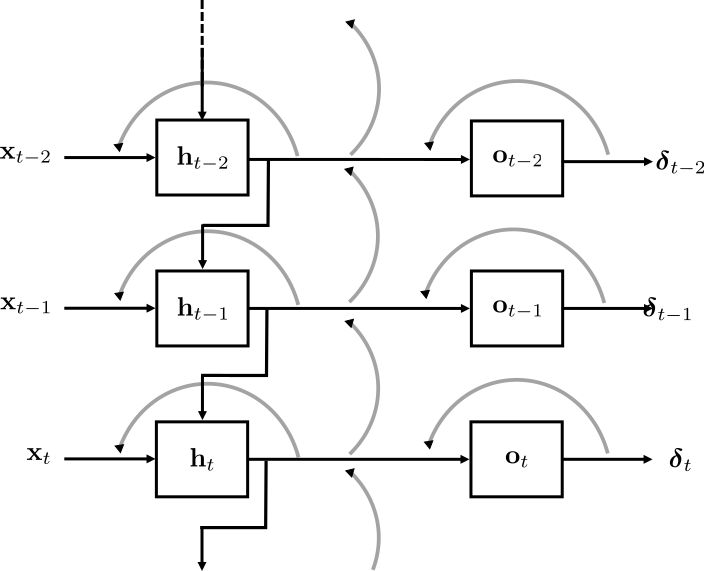
\includegraphics[scale=0.35]{Module 5 (RNN)/pics/smaller_rnn_unrolled_BP.pdf}
\columnbreak
\begin{itemize}
    \item The error term $\bdelta_t$ must be backpropagated through $\bW_{oh}$ in order to reach $\bW_{hx}$ at input $\bx_t$.
    \item It has to be repeatedly backpropagated through $\bW_{hh}$ in order to reach the input matrix at each one of the inputs $\bx_{t-t'}$.
\end{itemize}
\end{multicols}
\end{frame}

\begin{frame}{Derivation of the gradients}{Gradient with respect to the input weights}

To compute directly the gradient with respect to the weights, the chain rule must be used as follows. 
\begin{enumerate}
\item Compute the gradient  $\left(\nabla_{\bh_t} J_{ML}\right)$ of the cost function  respect to $\bh_t$. 
\item Compute the derivatives of the components of $\bh_t$ with respect to each component of $\bz_t^{(x)}$, which gives the derivative of the tanh activation. 
\item Compute the gradient of $\bz_t^{(x)}$ with respect to $\bW_{hx}$, which gives vector $\bx_t$. 
\end{enumerate}

\end{frame}

\begin{frame}{Derivation of the gradients}{Gradient with respect to the input weights}
    \begin{itemize}
        \item The product of these elements has to be written in the right order so the gradient has the same dimensions as matrix $\bW_{hx}$.
        \item The result is  
\begin{equation}\label{eq:gradient_hx}
\begin{split}
    \nabla_{\bW_{hx}} J_{ML} &=\sum_{t=1}^T \nabla_{\bW_{hx}}\bz^{(x)}_t  \left(\nabla_{\bh_t} J_{ML}\right)^\top \frac{\delta \bh_t}{\delta \bz^{(x)}_t}\\
    &=\sum_{t=1}^T \bx_t   \left(\nabla_{\bh_t} J_{ML}\right)^\top\diag\left( \tanh'\left(\bz^{(x)}_t\right) \right)
\end{split}
\end{equation}
where  the derivative of the hyperbolic tangent activation is  expressed as a Jacobian represented by a diagonal matrix. 
    \end{itemize}
\end{frame}
\begin{frame}{Derivation of the gradients}{Gradient with respect to the input weights}
\begin{itemize}
    \item A similar result can be found  for the biases 


\begin{equation}\label{eq:gradient_bias_h}
    \nabla_{\bb_{h}} J_{ML} =\sum_{t=1}^T    \diag\left( \tanh'\left(\bz^{(x)}_t\right) \right)\left(\nabla_{\bh_t} J_{ML}\right)
\end{equation}

    
\begin{equation}
    \nabla_{\bb_{h}} J_{ML} =\sum_{t=1}^T    \left(\nabla_{\bh_t} J_{ML}\right)^\top\diag\left( \tanh'\left(\bz^{(x)}_t\right) \right)
\end{equation}
\end{itemize}
\end{frame}

\begin{frame}{Derivation of the gradients}{Gradient with respect to the input weights}
\begin{itemize}
    \item The above equations have the  same form as any previously computed gradient: it is the product of
    \begin{enumerate}
    \item  the input sample $\bx_t$ as a column vector 
    \item a vector representing the backpropagated error
    \end{enumerate}
    \item The error is embedded in the (recursive) gradient with respect to the hidden state. This is, the error backpropagated to the input can be written as 
    $$\bdelta_t^{(bp)} = \diag\left( tanh'\left(\bz^{(x)}_t\right) \right) \left(\nabla_{\bh_t} J_{ML}\right)$$.
\end{itemize}
\end{frame}

\begin{frame}{Derivation of the gradients}{Gradient with respect to the hidden state weights}

For this set of weights, the backpropagation of the error at instant $t$

\begin{multicols}{2}
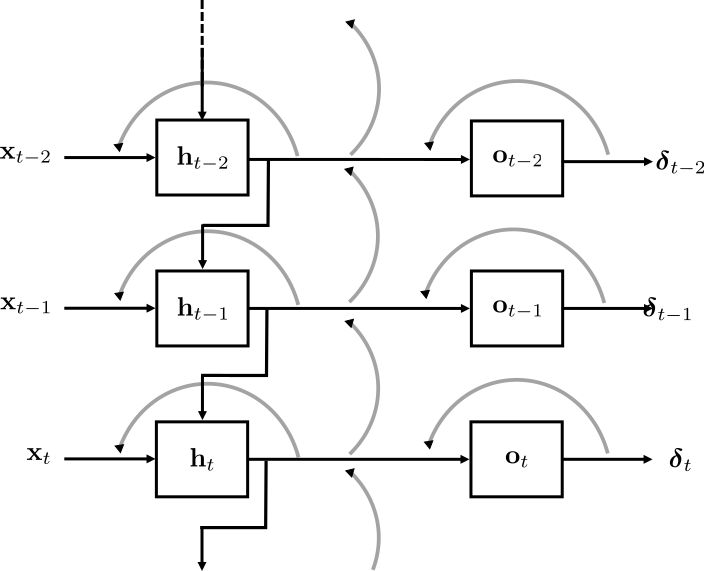
\includegraphics[scale=0.35]{Module 5 (RNN)/pics/smaller_rnn_unrolled_BP.pdf}
\columnbreak

    \begin{enumerate}
        \item Starts from the output $\bo_t$.
        \item It is transformed with output weights $\bW_{oh}$
        \item This error is used to update $\bW_{hh}$. The input is is $\bh_{t-1}$. 
        \item The backpropagation  then goes to the previous time instant, which requires another transformation of the error $\bW_{hh}$. 

    \end{enumerate}
\end{multicols}
\end{frame}


\begin{frame}{Derivation of the gradients}{Gradient with respect to the hidden state weights}
    \begin{itemize}
        \item 
To see this, we can compute the gradient  with respect to the hidden weights.
\begin{equation}\label{eq:gradient_hh}
\begin{split}
    \nabla_{\bW_{hh}} J_{ML} &=\sum_{t=1}^T \nabla_{\bW_{hh}}\bz^{x}_t  \left(\nabla_{\bh_t} J_{ML}\right)^\top \frac{\delta \bh_t}{\delta \bz^{(x)}_t}\\
    &=\sum_{t=1}^T \bh_{t-1}   \left(\nabla_{\bh_t} J_{ML}\right)^\top\diag\left( tanh'\left(\bz^{(x)}_t\right) \right)
\end{split}
\end{equation}
\item The gradient of $\bz_t$ is computed now with respect to $\bW_{hh}$.
\item The result is the input to these weights $\bh_{t-1}$.
\item This is known as backpropagation through time (BPTT). 
\item For $\bb_h$ , if we remove $\bh_{t-1}$ from \eqref{eq:gradient_hh}, we obtain the same result as in Eq. \eqref{eq:gradient_bias_h}. 
    \end{itemize}
\end{frame}

\begin{frame}{Summary of the backpropagation through time}
{Output weights}
    \begin{itemize}
        \item Compute the output errors $\bdelta_t$, $1 \leq t \leq T$.
        \item Use these errors to update the output weights with Eqs. \eqref{eq:gradient_oh} and \eqref{eq:gradient_o}.
\begin{equation}
\begin{split}
 \bW_{oh} &\leftarrow \bW_{oh} -\mu   \sum_{t=1}^T   \bh_{t}\bdelta_{t}^\top \\
 \bb_{oh} &\leftarrow \bb_{oh} -\mu   \sum_{t=1}^T   \bdelta_{t} \\
 \end{split}
\end{equation}
    \end{itemize}
\end{frame}

\begin{frame}{Summary of the backpropagation through time}
{Input weights and hidden state weights}
\begin{itemize}
    \item Compute the gradient with respect to the hidden states
    \begin{equation}\label{eq:gradient_h_t}
    \nabla_{\bh_t}J_{ML}=\bW_{oh}\bdelta_{t} + \bW_{hh}  \text{diag}\left(\text{tanh}'\left(\bz^{(x)}_{t+1}\right)\right)\left(\nabla_{\bh_{t+1}}J_{ML} \right)
\end{equation}
\item Update with Eqs. \eqref{eq:gradient_hx}, \eqref{eq:gradient_bias_h}, and \eqref{eq:gradient_hh}. 
\begin{equation}
\begin{split}
    \bW_{hx} & \leftarrow \bW_{hx} - \mu \sum_{t=1}^T \bx_t   \left(\nabla_{\bh_t} J_{ML}\right)^\top\diag\left( \tanh'\left(\bz^{(x)}_t\right) \right)\\
    \bb_{h} & \leftarrow \bb_{h} - \mu \sum_{t=1}^T \diag\left( tanh'\left(\bz^{(x)}_t\right) \right)\left(\nabla_{\bh_t} J_{ML}\right)
\end{split}
\end{equation}
\begin{equation}
    \bW_{hh} \leftarrow \bW_{hh} -\mu \sum_{t=1}^T \bh_{t-1} \left(\nabla_{\bh_t} J_{ML}\right)^\top  \diag\left( \tanh'\left(\bz^{(x)}_t\right) \right) 
\end{equation}
\end{itemize}
\end{frame}

\end{document}